\documentclass[paper=a4, fontsize=11pt]{scrartcl}
\usepackage[T1]{fontenc}
\usepackage{fourier}

\usepackage[english]{babel}															% English language/hyphenation
\usepackage[protrusion=true,expansion=true]{microtype}	
\usepackage{amsmath,amsfonts,amsthm} % Math packages
\usepackage[pdftex]{graphicx}	
\usepackage{url}
\usepackage{hyperref}


%%% Custom sectioning
\usepackage{sectsty}
\allsectionsfont{\centering \normalfont\scshape}
\usepackage{subfigure}

\usepackage{comment}


%%% Custom headers/footers (fancyhdr package)
\usepackage{fancyhdr}
\pagestyle{fancyplain}
\fancyhead{}											% No page header
\fancyfoot[L]{}											% Empty 
\fancyfoot[C]{}											% Empty
\fancyfoot[R]{\thepage}									% Pagenumbering
\renewcommand{\headrulewidth}{0pt}			% Remove header underlines
\renewcommand{\footrulewidth}{0pt}				% Remove footer underlines
\setlength{\headheight}{13.6pt}


%%% Equation and float numbering
%\numberwithin{equation}{section}		% Equationnumbering: section.eq#
%\numberwithin{figure}{section}			% Figurenumbering: section.fig#
%\numberwithin{table}{section}				% Tablenumbering: section.tab#


%%% Maketitle metadata
\newcommand{\horrule}[1]{\rule{\linewidth}{#1}} 	% Horizontal rule

\title{
		%\vspace{-1in} 	
		\usefont{OT1}{bch}{b}{n}
		\normalfont \normalsize \textsc{CS650 - Computer Vision} \\ [25pt]
		\horrule{0.5pt} \\[0.4cm]
		\huge Programming Lab 3 \\ Graph-cut Segmentation \\
		\horrule{2pt} \\[0.5cm]
}
\author{
		\normalfont 								\normalsize
        Daqing Yi\\[-3pt]		\normalsize
        \today
}
\date{}


%%% Begin document
\begin{document}
\maketitle

\section{Introduction}

A graph cut separates the vertices of a graph into two disjoint subsets.
A minimum cut is a graph cut that uses the smallest number of edges.
The problem can also be reduced to a maximum flow problem by the max-flow min-cut theorem~\cite{wiki:Max-flow_min-cut_theorem}.
By defining the source and the sink in a graph structure, the minimum cut can be used to solve the classification problem that minimizes a given energy function.

In a binary labeling problem, the pixels of an image should be labeled into either foreground or background.
After defining the source and the sink, a graph structure that represents both the inter-relationship between neighboring pixels and the likelihoods to be foreground and background can be constructed.
The minimum cut operation can segment the pixels into foreground and background which minimizes the energy function defined from the weighted edges of the graph structure~\cite{937505}.

In this lab, the code is written in C++.
Qt4.8 is used for the implement of GUI interaction.
The Vladimir Kolmogorov's C++ Implementation ( \emph{ maxflow-v3.03.src } ) is chosen for doing minimum cut.

\section{Graph Cut Segmentation}

% Smoothness Ratio 50
% Kernel Density Estimator Bandwidth 80
\begin{figure}[h]
\centering
\subfigure[Origin]{
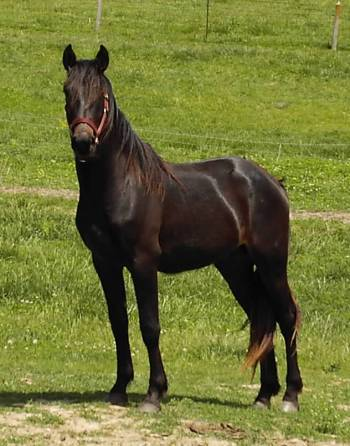
\includegraphics[width=.23\textwidth]{./figure/horse.jpg}
\label{fig:graph_cut:01:origin} }
\subfigure[Labeling]{
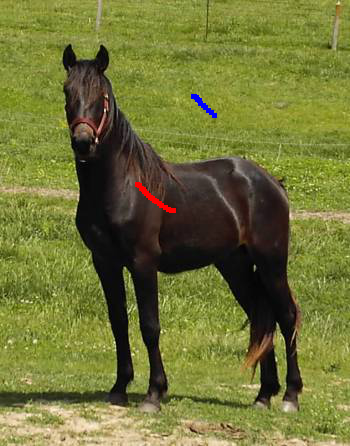
\includegraphics[width=.23\textwidth]{./figure/horse-label.png} 
\label{fig:graph_cut:01:labeling} }
\subfigure[Foreground mask]{
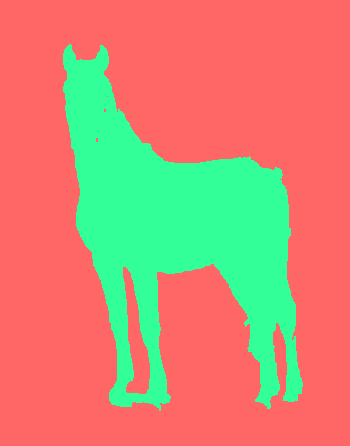
\includegraphics[width=.23\textwidth]{./figure/horse-mask.png} 
\label{fig:graph_cut:01:foreground_mask} }
\subfigure[Foreground cutted]{
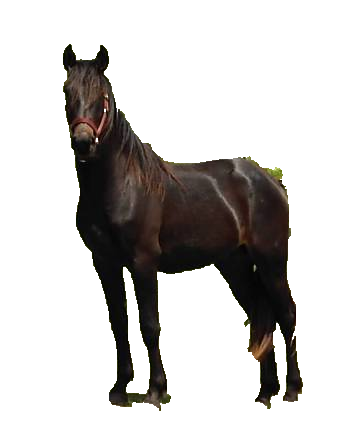
\includegraphics[width=.23\textwidth]{./figure/horse-foreground.png}
\label{fig:graph_cut:01:foreground} }
\caption{Graph cut segmentation on \emph{horse.jpg}. }
\label{fig:graph_cut:01}
\end{figure}

\begin{figure}[h]
\centering
\subfigure[Origin]{
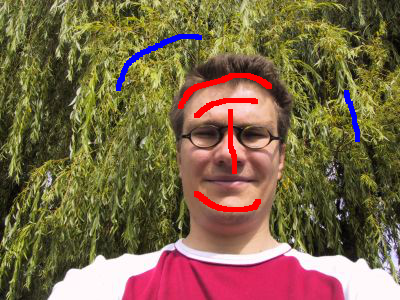
\includegraphics[width=.23\textwidth]{./figure/carsten-label.png}
\label{fig:graph_cut:02:labeling} }
\subfigure[Labeling]{

\includegraphics[width=.23\textwidth]{./figure/carsten-foreground2.png} 
\label{fig:graph_cut:02:less_smooth} } % smooth ratio 25
\subfigure[Foreground mask]{

\includegraphics[width=.23\textwidth]{./figure/carsten-foreground1.png} 
\label{fig:graph_cut:02:normal_smooth} } % smooth ratio 50
\subfigure[Foreground cutted]{
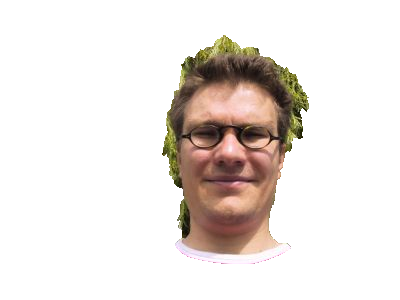
\includegraphics[width=.23\textwidth]{./figure/carsten-foreground3.png}
\label{fig:graph_cut:02:more_smooth} }  % smooth ratio 120
\caption{Graph cut segmentation on \emph{carsten.jpg}. }
\label{fig:graph_cut:02}
\end{figure}

\section{Grab Cut Segmentation}

\cite{rother2004grabcut}

Plot energy decrease

\begin{comment}
As before, prepare a write-up that describes your work.  Show examples of your code applied to different images.  What kinds of images does graph-cut segmentation (or Grab Cut respectively) work well for? What kinds of images do you find it struggles with? 
\end{comment}


\bibliography{reference}
\bibliographystyle{plain}

\end{document}